\section{Test på LEGO bil}

Gennem projektarbejdet, har vi testet den endelige løsning på LEGO-bilen. Men da simuleringen af det komplette digitale system med korrektion for steady state error ikke fungerede, er der kun testet med modellen for den kontinuere kontroller  med diskrete integrations blokke, så LEGO-computeren kan følge med beregningsmærssigt. Dette er ikke den helt optimale løsning, idet vi burde sample uendeligt hurtigt for at leve op til den kontinuere controller forventninger. Dog burde vores realisering, ligne vores simulering, hvor vi også har indført diskrete integrations blokke for at kunne sammenligne med bilens opførelse. Controlleren for LEGO bilen kan ses i \autoref{fig:Simulink_blokdiagram_LEGO} 

\begin{figure}[H]
	\centering
	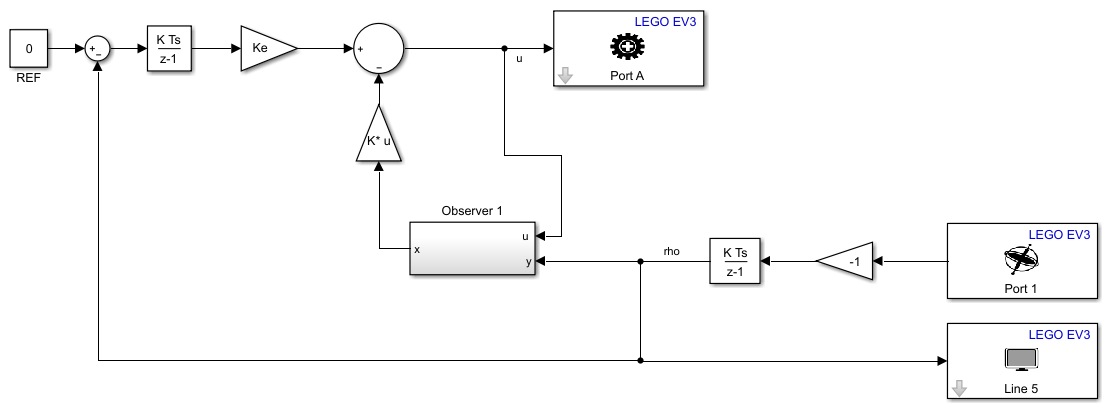
\includegraphics[width = 1\textwidth]{figur/Simulink_blokdiagram_LEGO}
	\caption{Blok diagram for den kontinuere controller uden observer}
	\label{fig:Simulink_blokdiagram_LEGO}
\end{figure}

Det ses i \autoref{fig:Simulink_blokdiagram_LEGO}, at outputtet måles af gyroskopet (vinkelhastighed) og integreres til en vinkel, inden det sendes ind i den kontinuere observer for at få states matricen ud. Gain blokken med -1 er for at vende gyroskopets signal rigtigt. LEGO bilen sender også vinklen rho ud på sin terminal så vi kan se den vinkel den måler, og hvor meget den drifter med tiden.

Under realiseringen, opdagede vi dog endnu en fejlkilde, som gjorde at systemet opførte sig anderledes. Dette kom af den friktion som systemet har. Denne friktion er nemlig ikke lineær, hvilket betyder, at modstanden falder, når spændingen til motoren når en bestemt størrelse. Derfor får systemet et kraftigt udsving, da den overkompenserer for en fejl. Projektet har derfor et realiserings problem, og vil skulle bruge en meget hurtig regulerings sløjfe, for at kunne korrigere for fejlen. Dette er nok ikke muligt i praksis, hvorfor en bedre løsning ville være at indføre 2 systemer. Her ville det første system, have kontrol over motoren, når friktionen er statisk, og det andet system tager over, når friktionen bliver dynamisk og modstanden falder.

På \autoref{fig:lego_bil} vises et billede af realiseringen, hvor aksen med hjulene står med en skæv vinkel, mens at aksen med kroppen af bilen, står vandret. 

\begin{figure}[H]
	\centering
	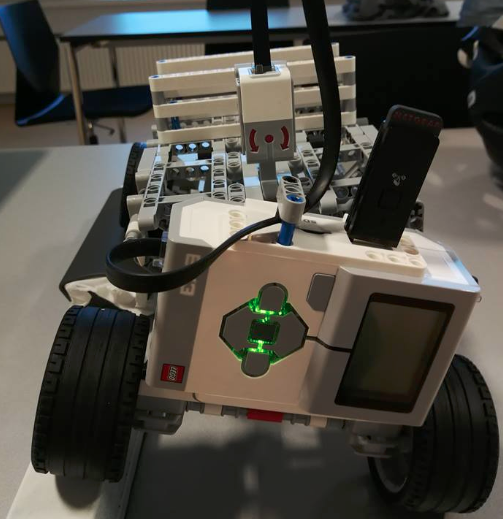
\includegraphics[width = 300pt]{figur/lego_bil}
	\caption{Lego realisering}
	\label{fig:lego_bil}
\end{figure}   

Bilen kan godt regulere sig ind til vandret, hvis den ikke bliver påført en for stor forstyrrelse fx en vinkel over 20-30 grader. Bliver vinklen for stor overkompenserer bilen pga. friktion. Bilen virker også kun i nogle ganske få minutter, da gyroskopet derefter har driftet og viser forkert vinkel, hvilket for bilen til at overkompensere endnu mere, da vandret nu er "forskudt". Til sidste er systemet ikke glad for hurtige ændringer, da dette får gyroskopet til at drifte hurtigere.